\documentclass[a4paper, 12pt, one column, aas_macros]{article}

%% Language and font encodings. This says how to do hyphenation on end of lines.
\usepackage[english]{babel}
\usepackage[utf8x]{inputenc}
\usepackage[T1]{fontenc}
\usepackage{aas_macros}

%% Sets page size and margins. You can edit this to your liking
\usepackage[top=1.3cm, bottom=2.0cm, outer=2.5cm, inner=2.5cm, heightrounded,
marginparwidth=1.5cm, marginparsep=0.4cm, margin=2.5cm]{geometry}

%% Useful packages
\usepackage{graphicx} %allows you to use jpg or png images. PDF is still recommended
\usepackage[hyphens]{xurl}
\usepackage[colorlinks=False]{hyperref} % add links inside PDF files
%\usepackage{breakurl}
\usepackage{amsmath}  % Math fonts
\usepackage{amsfonts} %
\usepackage{amssymb}  %
\usepackage[section]{placeins} % Add float barrier at start of each new section

%% Citation package
\usepackage[authoryear]{natbib}
\bibliographystyle{abbrvnat}
\setcitestyle{authoryear,open={(},close={)}}


\title{Exploring Procedural Generation Algorithms in \\Unity 2D}
\author{Ryan Overbeck}

\begin{document}
\maketitle


\tableofcontents


\section{Introduction}
Procedural generation has become a vital tool in modern game development, allowing developers to efficiently create expansive, varied, and engaging virtual environments. This paper explores three distinct procedural generation algorithms implemented within Unity's 2D framework: Binary Space Partitioning (BSP), Random Walk, and Wave Function Collapse (WFC). Each algorithm provides a unique approach and set of advantages, particularly when applied to generating dungeon layouts for games.

The Binary Space Partitioning method subdivides a given space iteratively to generate structured, room-based dungeons. Conversely, the Random Walk method leverages random processes to produce more organic, winding paths. The Wave Function Collapse algorithm, inspired by concepts from quantum mechanics, systematically applies adjacency constraints to generate coherent tile-based layouts. By examining these algorithms, this paper not only documents their implementation specifics and practical considerations but also evaluates the challenges faced when integrating these techniques into Unity's environment. The project's complete source code is publicly available at \url{https://github.com/rjoverbeck/procgen-dungeon}.

\section{Project Setup}
To integrate our three dungeon-generation approaches with Unity's rendering pipeline, we implement a single class, \texttt{TilemapGenerator} (which inherits from \texttt{MonoBehaviour}) which drives tile placement from any of the position generators. Each generator---Binary Space Partitioning, Random Walk, and Wave Function Collapse---exposes a \texttt{Generate(...)} method returning a \texttt{Queue<Vector2Int>} of floor-tile coordinates. The \texttt{TilemapGenerator} then consumes this queue to draw tiles onto a Unity \texttt{Tilemap} over time, updating a simple UI counter as it goes.

To enable interactive exploration and real-time comparison of the three procedural methods, we attach a \texttt{PlayerMovement} component to the player character. This component implements \texttt{Controls.IGameplayActions} from Unity's Input System: the \texttt{OnMove} callback reads a \texttt{Vector2} from the \texttt{Move} action each frame and applies it to the player's \texttt{Rigidbody2D} (scaled by \texttt{moveSpeed}) for smooth movement. Additionally, three input callbacks---\texttt{OnCreateBSPTilemap}, \texttt{OnCreateRWTilemap}, and \texttt{OnCreateWFCTilemap}---are bound to dedicated keys or buttons. When the player presses the corresponding control, the script invokes \texttt{tilemapGenerator.CreateBSPTilemap()}, \texttt{CreateRWTilemap()} or \texttt{CreateWFCTilemap()}, respectively. This design lets the player freely traverse the current dungeon layout and, at any moment, regenerate the floor using the BSP, Random Walk, or WFC algorithm, facilitating immediate, in-game comparisons of each procedural style.

\section{Binary Space Partitioning Approach}
\subsection{Introduction}
\begin{quote}
  \emph{"A binary space partition takes a given space and splits it in half, and then takes the two areas that were created and splits those in half, and repeats until some threshold is reached."}
  \cite[p.~293]{ShortAdams2017}
\end{quote}

This quote sums up our first approach to procedurally generate rooms for our 2D dungeon. In this implementation, we define a rectangular region---the entire dungeon area---and iteratively subdivide it into smaller rectangles (potential ``rooms'') until no further meaningful subdivision is possible. Lastly, some offset is applied to create space between these rooms. The following outlines how this Binary Space Partitioning approach is handled in our Unity project.

\subsection{Setting up the Initial Partition}
The process begins by defining a single large bounding area using a \texttt{BoundsInt} structure. As noted in the Unity documentation, the \texttt{BoundsInt} structure ``represents an axis aligned bounding box with all values as integers'' \citep{unity_docs}. This is useful for several reasons, among them since \texttt{BoundsInt} uses integer coordinates, it aligns naturally with tile-based systems (where tiles or grid cells are also defined by integral x, y positions).

Next, this bounding area is enqueued in a \texttt{Queue<BoundsInt>} which manages partitions that still need to be processed. A queue-based approach was selected to keep the partitioning logic simple and easy to follow. A stack-based approach would have worked equally as well---only changing the order of processing.

\subsection{Iterative Subdivision}
While there are partitions in the queue:
\begin{itemize}
  \item Dequeue the next partition.
  \item Check if the current partition meets or exceeds the \emph{minimum width} (\texttt{minWidth}) and \emph{minimum height} (\texttt{minHeight}) constraints.
  \item If it can be subdivided, choose randomly whether to \emph{prefer a horizontal} or \emph{vertical} split (a 50/50 chance). Attempt to partition the space along that orientation if there is sufficient size to do so at least twice (e.g., if the height is at least \texttt{2 * minHeight} for a horizontal split).
  \item If the chosen orientation is not feasible, try the alternative orientation.
  \item If neither orientation is possible (the partition is too small), mark that partition as finalized (a ``room'') and add it to the \texttt{partitions} list.
\end{itemize}

\subsection{Managing Subdivisions}
The actual subdivision is performed in two helper methods, \texttt{PartitionHorizontally} and \texttt{PartitionVertically}. These methods randomly determine a \emph{split point} within the valid range and create two new \texttt{BoundsInt} objects representing the subdivided spaces. Each new partition is enqueued for further subdivision if possible.

\begin{itemize}
  \item \emph{Horizontal Partition:} Splits along the y-axis, producing a top and bottom rectangle.
  \item \emph{Vertical Partition:} Splits along the x-axis, producing a left and right rectangle.
\end{itemize}

By randomly selecting either horizontal or vertical splits (with both given equal chance), the algorithm produces layouts of different shapes, preventing overly predictable results.

\subsection{Applying Offset}
Once the BSP iterations have yielded a queue of bounding boxes, the method \\ \texttt{GetPositionsFromPartitions} converts these spatial chunks into concrete tile coordinates while honouring a configurable margin. Its behaviour can be summarised in four concise steps:
\begin{enumerate}
  \item A \texttt{Queue<Vector2Int>} is created to hold every interior grid coordinate that will ultimately be used by the tilemap.
  \item For every bounding box in the collection, the method scans the rectangle column-wise. Two nested loops sweep the integer ranges 
\[
\begin{aligned}
  x &\in [\,\text{\texttt{partitionOffset}},\;
           \text{\texttt{partition.size.x}}
           - \text{\texttt{partitionOffset}}) \\[4pt]
  y &\in [\,\text{\texttt{partitionOffset}},\;
           \text{\texttt{partition.size.y}}
           - \text{\texttt{partitionOffset}})
\end{aligned}
\]
thereby discarding a border of thickness \texttt{partitionOffset} on all four sides. This margin separates the bounding boxes into rooms.
  \item Each local offset \texttt{(x,y)} is converted to an absolute grid coordinate by adding it to \texttt{partition.min}. Because \texttt{partition.min} stores the rectangle's lower-left corner, the expression \texttt{(Vector2Int)partition.min + new Vector2Int(x,y);} yields the true position that the tile will eventually occupy in the global tilemap.
  \item The method finally returns the populated \texttt{positions} queue, providing a collection of draw-eligible positions from the bounding boxes constructed by BSP.
\end{enumerate}

\subsection{Conclusion}
By combining a straightforward queue-based BSP algorithm with configurable size thresholds and offsets, we achieve a flexible grid-like room-layout generator. The approach naturally produces a range of room shapes and sizes and easily adapts to different dungeon dimensions. Moreover, isolating the subdivision logic into small helper methods keeps the code base clean and maintainable. Overall, Binary Space Partitioning proved to be a reliable foundation for our 2D dungeon generation, and provided a foundation for exploring other procedural content generation techniques.

\section{Random Walk Approach}
\subsection{Introduction}
\begin{quote}
  \emph{"Random walks are produced by starting at a given point and then taking steps in random directions. Many natural processes, like molecular  motion, can be described by random walks, and they can be useful for  generating all sorts of naturalistic paths and features."}
  \cite[p.~286]{ShortAdams2017}
\end{quote}

This quote sums up our second approach to procedurally generate rooms for our 2D dungeon. In this implementation, we choose a starting position and perform a defined number of ``walks,'' each consisting of a certain number of steps. Every time we move to a new position, we record that position in a set of coordinates. After all walks are completed, these coordinates form the layout of our dungeon floor. The following outlines how this is handled in our Unity project.

\subsection{Initial Conditions}
A \texttt{HashSet} is initialized to keep track of every visited position (avoiding duplicates).

\subsection{Iterations (Walks)}
The number of iterations (walks) is determined by an input parameter. For each walk:
\begin{itemize}
  \item A \texttt{Vector2Int} for storing the previous position is set to the start position (provided by an input parameter).
  \item Perform a fixed number of steps, where each step is taken in a randomly chosen direction (up, down, left, or right). The new position after each step is added to the set, and the previous position is updated.  
\end{itemize}

\subsection{Results}
After all walks and steps are completed, the algorithm returns the set of all unique positions visited during the random walk.

\subsection{Conclusion}
The Random Walk approach offers a highly organic alternative to the grid-like BSP rooms. By adjusting \texttt{walkCount} and \texttt{stepCount}, one can fine-tune corridor density (i.e. the number of gaps between paths), branching complexity (i.e. the number of turns in a path), and overall coverage (i.e. the number of gaps overall). Its simplicity and reliance on basic data structures make it easy to integrate and experiment with in Unity, providing rapidly generated, exploratory dungeons that contrast sharply with the more predictable, room-oriented layouts of the BSP method.

\section{Wave Function Collapse Approach}
\subsection{Introduction}
The Wave Function Collapse (WFC) algorithm, specifically the Simple Tiled variant is a procedural generation method that draws inspiration from quantum mechanics to create tile-based patterns. It works by assigning a set of potential states to each tile and then progressively reducing these possibilities based on constraints from adjacent tiles, much like the collapse of a quantum state into a definite outcome. 

A simplified version of this algorithm (without support for tile symmetry e.g. rotations or reflections) forms the third approach for generating the layout of our dungeon. Its implementation in our Unity project is explored below.

\subsection{Setting up}
\subsubsection{Adjacency Constraints}
The first step in setting up the algorithm is to establish valid tile adjacencies for the supplied tileset. To ensure the tiles tile appropriately, every pair of adjacent pixels on the edge of neighboring tiles must be the same color (see figure \ref{fig:wfc-tile-adjacency-constraints}). To that end, the method \texttt{GetTilesEdgesColors} accepts a list of tiles which are of the type \texttt{Texture2D} (representing bitmaps), it then extracts and returns the color information for every pixel along each tile's edge.

\begin{figure}[htbp]
  \centering
  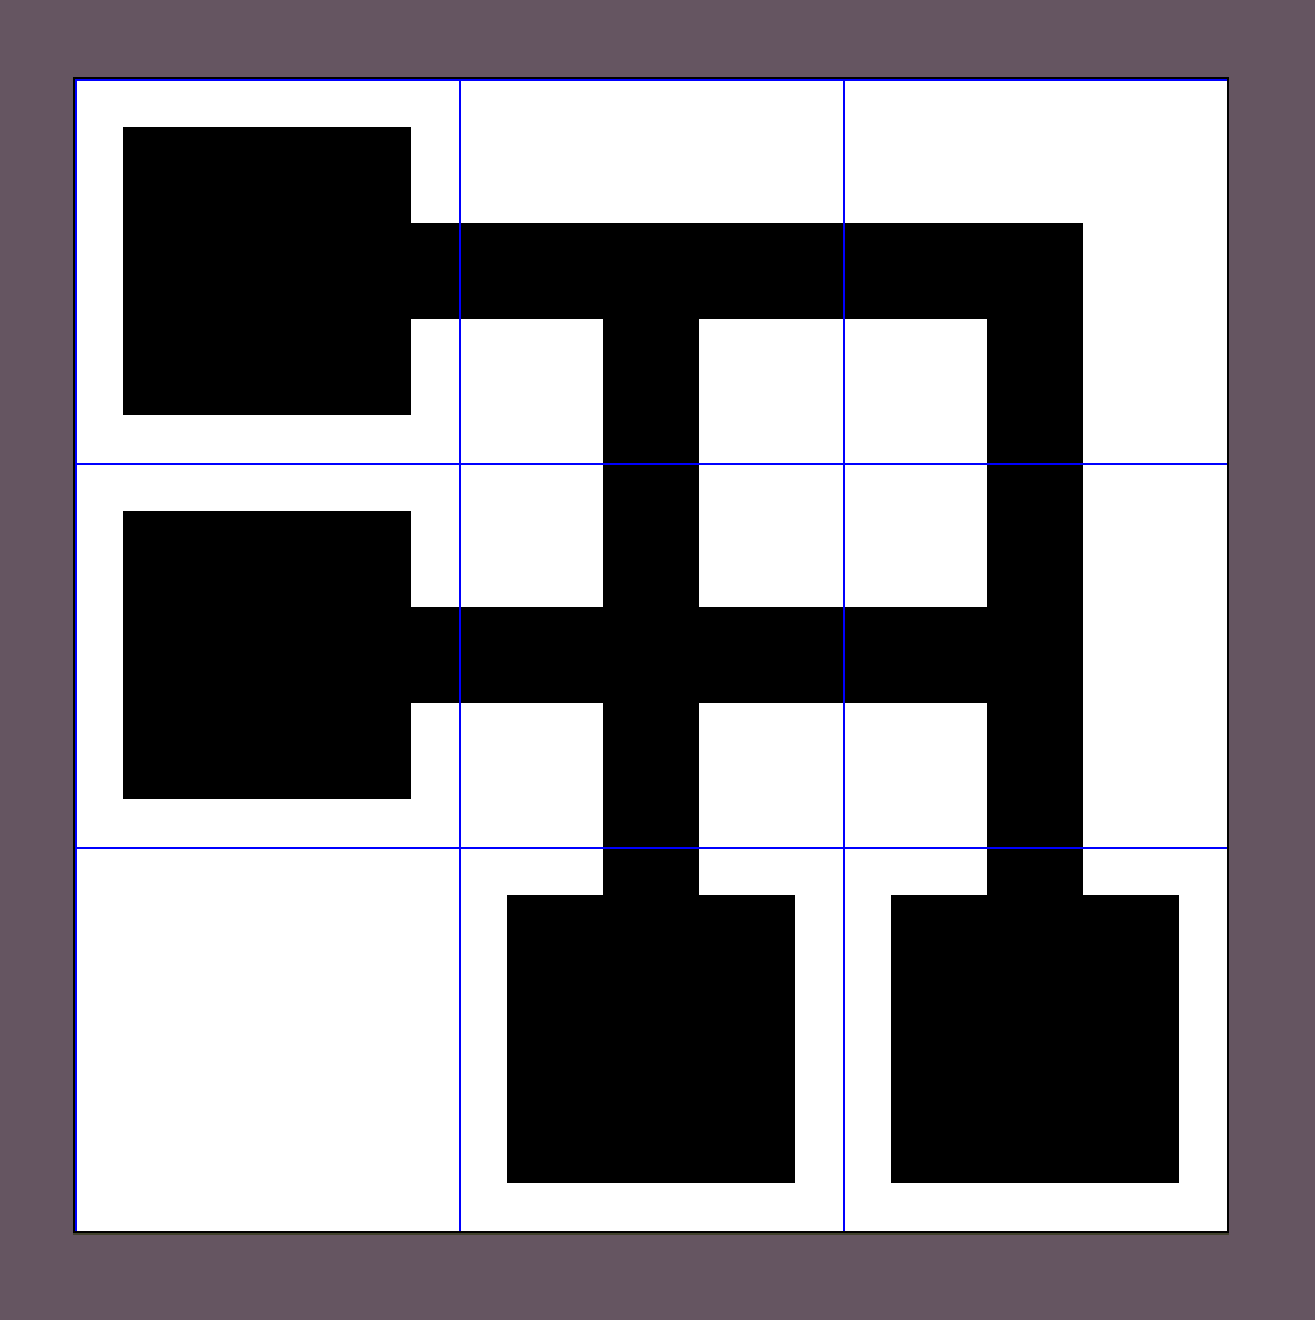
\includegraphics[width=0.7\textwidth]{images/wfc-tile-adjacency-constraints.png}
  \caption{Tile Adjacency Constraints}
  \label{fig:wfc-tile-adjacency-constraints}
\end{figure}

\subsubsection{Finding Viable Tiles for each Tile's Edge}
The next step is to determine for each tile which tiles satisfy the adjacency constraints. The method \texttt{GetTilesEdgesViableTiles} performs this task by iterating through each tile and examining every one of its four edges. For each edge, the method identifies its complementary edge (i.e., the bottom edge is compared with the top edge, and the left edge with the right edge) using a helper function \texttt{GetComplementaryEdge}.

The method then compares the colors of the current edge with the corresponding complementary edge of every tile by using a pixel-by-pixel comparison via the \texttt{EdgesMatch} helper function. If the two edges match exactly, the index of the candidate tile is recorded as a viable neighbor. This process results in a three-dimensional array where each element contains the list of tile indices that can be placed adjacent to a given tile on a specific edge.

This step is crucial as it ensures that only tiles with matching edge colors are considered for adjacent placement, thus maintaining the seamless appearance of the tiled pattern.

\subsubsection{Mapping Tiles to Weights}
The function \texttt{GetTilesToWeights} is responsible for constructing a dictionary that maps each tile's identifier (an integer index) to its corresponding weight. These weights, provided in the \texttt{tileWeights} list---sourced to a serialized field in the Inspector---can be interpreted as the desirability of selecting a given tile during the cell collapse process. Since it is assumed the weights are in order, the method iterates up to the number of tiles. At each step, it adds a new key-value pair to \texttt{tilesToWeights}, using the loop index as the key and \texttt{tileWeights[i]} as the value. Once the loop completes, the fully populated dictionary is returned for each cell to use when initializing its set of viable (possible) tiles.

\subsubsection{Cell Structure and Entropy Calculation}
The \texttt{Cell} class encapsulates the state of each grid cell. Each cell maintains a dictionary (\texttt{viableTilesToWeights}) that reflects the current set of possible tiles along with their weights. Crucially, the cell also stores a computed value called \texttt{entropy}. In this context, entropy is a measure of uncertainty or randomness over the set of viable options, computed using the Shannon entropy formula:
\begin{equation}
  H(X) \;=\; -\sum_{i=1}^{n} p(x_i)\,\ln p(x_i)
\end{equation}

\subsubsection{Grid Initialization}
The function \texttt{InitializeOutputGrid} is tasked with constructing the overall grid that represents the output of this procedural generation algorithm. The grid is implemented as a dictionary where each key is a two-dimensional coordinate (represented by a \texttt{Vector2Int}) and the value is an instance of the \texttt{Cell} class.

\subsection{The Algorithm}
The algorithm is driven by the \texttt{CollapseCells} method which for every cell in the grid:
\begin{enumerate}
  \item Collapses the minimum-entropy cell.
  \item Enqueues that cell for neighbor-constraint propagation.
  \item Dequeues cells one by one, and for each of the four cardinal neighbors:
    \begin{itemize}
      \item Skips neighbors outside the grid or already collapsed.
      \item Builds the set of \emph{allowed} neighbor tiles by looking up, for each currently viable tile in the source cell, which adjacent tiles are compatible on the shared edge (using \texttt{tilesEdgesViableTiles[tile][edge]}).
      \item Prunes any tiles from the neighbor's \texttt{viableTilesToWeights} that are not in this allowed set.
      \item If the neighbor's viable set becomes empty, returns \texttt{true} to signal a contradiction (the process must be repeated).
      \item Otherwise, if pruning reduced its size, enqueues the neighbor for further propagation.
    \end{itemize}
\end{enumerate}

By iteratively collapsing low-entropy cells and propagating adjacency constraints, this method enforces global consistency across the grid or detects unsatisfiable configurations. If a contradiction is found, the grid is re-initialized and the process repeats.

\subsection{Extracting Tilemap Positions}
The function \texttt{GetPositionsFromGrid} takes the fully collapsed \texttt{outputGrid} and the list of source tile textures, and produces a \texttt{Queue<Vector2Int>} like the other position generators. It does so by iterating over every pixel within each cell's tile (\texttt{Texture2D}): if the sampled \texttt{Color} has red, green, and blue channels all equal to zero (i.e.\ pure black), the pixel represents a floor tile and can be added to the tilemap. The method computes the absolute tilemap position by scaling the cell's grid coordinate by the tile dimensions and adding the pixel offset.

\subsection{Conclusion}
Wave Function Collapse merges local adjacency rules with global constraint propagation to produce richly varied, coherent patterns that neither purely random methods nor rigid partitioning can achieve alone. Although its setup---defining edge-matching rules, weights, and entropy calculations---requires more upfront work, WFC excels at generating highly detailed, non-repeating dungeon layouts. Integrating this method into Unity demonstrated both the power of constraint-based generation and the importance of efficient propagation logic. As a result, WFC stands as a versatile third pillar in our procedural toolkit, complementing the structured rooms of BSP and the organic paths of Random Walk.

\section{Difficulties}
\subsection{Challenges in Adapting WFC to Unity}
The Wave Function Collapse (WFC) algorithm offers an innovative approach to procedural content generation. However, adapting it to a Unity 2D project presented several challenges, primarily due to shortcomings in the primary reference, the source for it on GitHub. \citep{mxgmn}

A major source of difficulty was the repository's README, which conflates two distinct variants of the algorithm: \emph{Simple Tiled} and \emph{Overlapping}. The failure to clearly differentiate between these variants led to confusion in the description of the algorithm which was crucial for reasoning about the source code due to poor naming conventions, lack of inline documentation, and terminology borrowed from Quantum Mechanics despite a tenuous connection.

This was not a unique difficulty, as one researcher noted, ``in personal correspondence with several users of WFC, we learned that many of them treated the code as a black box''. \citep{karth}

Beyond documentation-related difficulties, practical implementation introduced additional hurdles. One critical issue was my initial omission of an \texttt{isCollapsed} flag within the \texttt{Cell} structure. Without this flag, the algorithm repeatedly selected the first collapsed cell---which inherently possesses the lowest possible entropy (0)---thus preventing the correct progression through the grid.

Additionally, my original implementation incorrectly assumed a top-left origin for grid coordinates, resulting in a mismatch with Unity's coordinate system. This discrepancy caused a flawed mapping from the generated output grid to the intended tilemap.

Lastly, the propagation logic initially only addressed immediate cardinal neighbors of a collapsed cell. In practice, however, correct functionality necessitated iterative propagation through all affected neighbors to ensure adjacency constraints properly influenced the entire grid, thereby enabling information to ripple out and achieve global coherence.

\subsection{Challenges in Moving to Tile Generation Over Time}
When the project first aimed to generate a dungeon floor, the tile placement occurred synchronously on \texttt{Start()}. This approach was straightforward to implement but lacked any concept of observable progression over time. Addressing this necessitated several changes. 

First, the original data structure for storing the positions of the floor tiles, a \texttt{HashSet}, needed to be changed so that order could be preserved. Using a \texttt{Queue} was necessary to maintain first-in-first-out order. However, this change introduced a new challenge: since a \texttt{Queue} alone does not handle duplicates, a separate \texttt{HashSet} had to be used in parallel to record visited positions for algorithms that produced duplicates. By checking against this \texttt{HashSet} before enqueueing a new coordinate, the system could retain an ordered structure while still preventing repeated tiles from being added. Note that while Unity's \texttt{Tilemap.SetTile} method can handle duplicates it would obfuscate how the room is constructed over time so it became necessary to deal with them here.

Second, switching from a synchronous approach to an incremental, time-based approach introduced the need for coroutines. Previously, the entire tile set could be drawn in a single loop, effectively blocking until all positions were placed. In contrast, placing one tile every five milliseconds (as is the speed currently) requires the code to yield partway through execution so that the game loop can continue running. Implementing the coroutine \texttt{DrawFloorTilesOverTime} allowed each tile placement to be spaced out over time without freezing the entire game.

Third, as tiles were placed over time, it became important to communicate the dungeon generation's progress to the player. A simple UI element was introduced to display both the total number of tiles to be placed and the number of tiles already placed, updating in real time as new positions were set.

In the original approach, all floor tiles appeared at once on game start (see figure \ref{fig:difficulty-1-before}), offering no indication of the generation process. With the revised approach, tiles are placed incrementally allowing the player to watch the dungeon emerge piece by piece (see figure \ref{fig:difficulty-1-after}).

\begin{figure}[htbp]
  \centering
  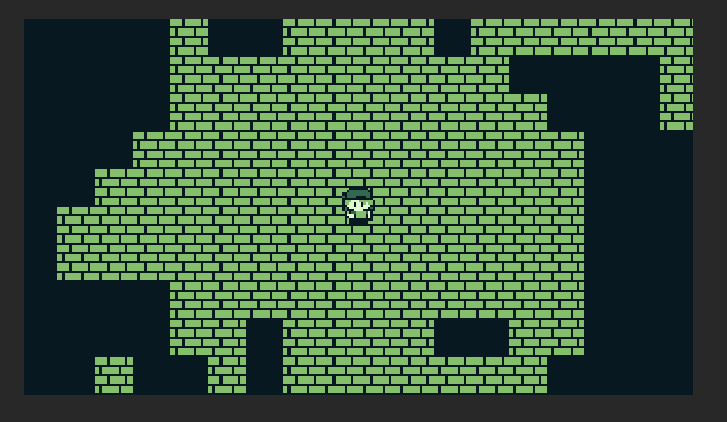
\includegraphics[width=0.7\textwidth]{images/difficulty-1-before.png}
  \caption{Challenge 4.1 - game view before}
  \label{fig:difficulty-1-before}
\end{figure}

\begin{figure}[htbp]
  \centering
  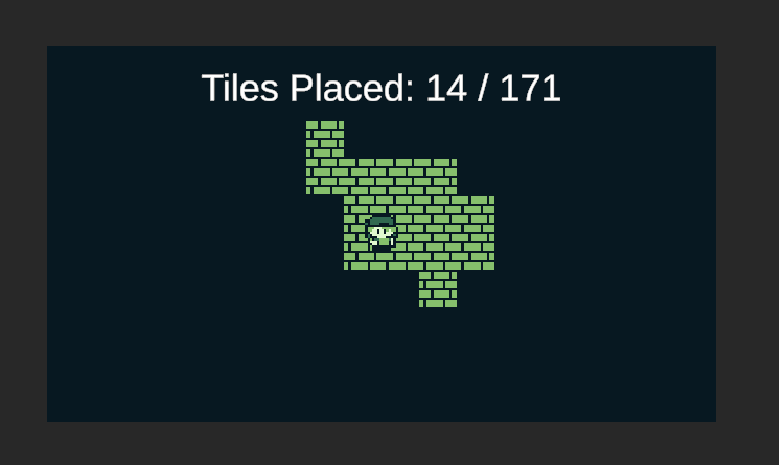
\includegraphics[width=0.7\textwidth]{images/difficulty-1-after.png}
  \caption{Challenge 4.1 - game view after}
  \label{fig:difficulty-1-after}
\end{figure}

\section{Impact of Previous Courses on Project}
\subsection{CSCI 451 and Utilizing Unity Coroutines}
Threads in C\# represent an operating-system-level construct. As stated by Silberschatz \emph{et al.}, ``A thread is a basic unit of CPU utilization; it comprises a thread ID, a program counter, a register set, and a stack'' \cite{silberschatz}. This means that each thread is scheduled independently by the operating system and can take advantage of multiple processor cores for true parallelism. However, the creation and management of multiple threads can be resource-intensive, and programmers must carefully manage data shared between threads to avoid race conditions. 

Unity coroutines, on the other hand, are not scheduled by the operating system. They are functions ``that can be suspended, resumed, and executed cooperatively (often on the same thread)'' \cite{nosenko}. In Unity, coroutines primarily run on the main thread and yield control voluntarily, allowing the engine to manage when to resume them. This cooperative model avoids the complexity of thread synchronization, but it does not offer true parallelism by default. Coroutines are particularly useful for tasks that must be broken into incremental steps across frames, such as animations or in the case of this project, long-running operations where you do not want to block the main thread.

My understanding of these concurrency mechanisms was greatly enhanced by taking \textit{CSCI 451 Operating Systems}. The course covered core concepts of processes, threads, synchronization, and CPU scheduling, providing the theoretical background to appreciate how the operating system manages threads and why threads are relatively expensive compared to language-level, cooperative concurrency mechanisms like coroutines. By exploring concurrency at the OS level first, it enables deeper insight into how coroutines abstract these complexities and thus offer a simpler model for many game development scenarios.

\subsection{WRIT 102 and Academic Sourcing/Technical Writing}
In addition to technical courses, the project benefited significantly from the skills acquired from University Studies, such as \textit{WRIT 102 Introduction to Academic Writing}. This course, which emphasized careful analysis, systematic research, and the construction of coherent academic arguments laid a solid groundwork for both identifying credible resources and organizing this paper effectively.

The techniques learned in \textit{WRIT 102} proved instrumental during the research phase by facilitating the systematic identification and evaluation of academic sources that supported the project. Moreover, the course's focus on proper documentation and citation ensured that all referenced materials were integrated seamlessly and accurately, thereby maintaining the academic integrity of the paper.

Lastly, the critical reading and persuasive writing strategies honed in the course helped in articulating complex technical concepts clearly and persuasively, bridging the gap between technical content and academic presentation.

\section{Conclusion}
Procedural content generation significantly streamlines the creation of complex and engaging game environments. Throughout this project, we explored three procedural generation algorithms---Binary Space Partitioning, Random Walk, and Wave Function Collapse---each offering distinct benefits and limitations. BSP provided clear, organized room structures, while Random Walk offered unpredictability and a natural flow, and WFC ensured complex, constraint-driven coherence. Integrating these algorithms into Unity's 2D environment highlighted practical challenges, such as coordinate system mismatches and managing tile placements over time.

Furthermore, the project underscored the importance of rigorous iterative testing, which was essential in overcoming implementation difficulties. Finally, the project's development and documantation were both significantly enriched by previous coursework whether it be in operating systems to understand concurrency or in technical writing to evaluate references.

This experience was invaluable as my Capstone project. It allowed me to synthesize and apply knowledge from multiple courses, provided hands-on exposure to algorithmic thinking and software development practices, and significantly deepened my understanding of procedural generation techniques. Ultimately, this project not only enhanced my technical proficiency but also prepared me for future challenges and innovations within the broader field of game development and computer science.

\bibliography{references}
\end{document}